% Drawing 148/02-10 -- folder 148, batch 02, archive page 30 (PDF page 31).
% Transcription: les dessins de la planche : une petite sphère pour chacun des neuf types, portant cinq points, avec équateur et méridiens --- $\mathrm{I}_{10}$, $\mathrm{I}_{6}$, $\mathrm{I}_{4}$ en haut ; $\mathrm{II}_{2}$, $\mathrm{II}'_{2}$ (précédée d'une sphère hachurée), $\mathrm{II}_{1}$ au milieu ; $\mathrm{III}_{2}$, $\mathrm{III}_{1}$ et $\mathrm{III}'_{2}$ en bas, ces deux dernières égalées chacune à une seconde sphère ; en marge gauche, trois petits graphes (un sommet à cinq arêtes libres ; deux sommets reliés portant trois et deux arêtes libres ; trois sommets en chaîne portant deux, une et deux arêtes libres).
% Kind: plate: the nine special five-point structures as small spheres, three marginal graphs. Method 2 (redraw from the facsimile). Status: partial.
% Notes: Redrawn from the colour scan (crops at 450 dpi), sphere by sphere: the pencil outline, the equator (front solid, back dashed), the meridian circles or oblique bands with their solid and dashed halves in the colours of the page (dark brown ink, orange-red), and every marked point placed where it stands on the page, with its label. I_10: five points on the equator (two behind, three in front). I_6: poles, the centre of the back, two points on the front equator, a meridian circle and a dashed axis. I_4: apex, two points behind and two in front, four meridian arcs (two solid, two dotted). II_2: narrow meridian circle, points alpha, alpha' behind and P, beta, beta' in front. The sphere before II'_2 is hatched over with oblique strokes (struck): drawn in grey with seven hatching strokes. II'_2: alpha, beta', P, beta, alpha_1, heavy right outline, meridian circle. II_1: heavy meridian oval through 1 and infinity, orange equator with the points read as u_5, u_4, u_3 behind and u_0, u_1, u_2 in front, a dashed axis, and 0 and P at the foot (an overinked blot above P is left out). III_2: two meridian bands, five brown points (two behind, three in front, the middle one P) and four dark crossing points. III_1 and III'_2: heavy outline arc, two oblique bands, short heavy and dotted strokes to the labelled points (P, P-bar, 0, infinity, 1; and P, alpha, alpha', beta, beta'); each is followed by « = » and a second sphere with equator and two meridian bands carrying the same labels. The three marginal graphs: one vertex with five legs; two joined vertices with three and two legs; three vertices in a chain with two, one and two legs. The name of each type is set above its sphere. Left out: all the text between the spheres (counts, groups, the degree arrows and their labels), the small curled arrows beside I_4 and the last sphere, two small pencil arrows on II'_2. Still differs: circles and bands are drawn as true ellipses fitted to the freehand ones (within about half a unit); on III'_2 two labels are overwritten on the page (alpha' over a beta, and the lower beta) and are given as finally written; the labels u_i of II_1 are a reading; the legs of the third marginal graph are placed from a small view. The notes of the transcription on the points of II_2, on « deux sphères ; la première est hachurée » and on « deux sphères égalées » describe parts of this plate. Redrawn 2026-11-12 (issue 128): to check again.
% Coordinates: 1 unit = 1 mm = 1/100 of the crop width, y downwards as on the crop (bbox in page fractions: [0.09, 0.07, 0.93, 0.455]).
% Redrawn by Claude (claude-fable-5-2), issue #128, 2026-11-12, from the colour scan at 350 dpi; not checked by a human; not compiled (no TeX in the session).
% Rights: reproduces part of the work -- behind RENDER_TRANSCRIPTS, never published by itself.
\documentclass[tikz,border=3pt]{standalone}
\usepackage{amsmath,amssymb}
\usetikzlibrary{patterns,arrows.meta}
\tikzset{pencil/.style={black!45}, struck/.style={black!35}, mpt/.style={circle,draw,inner sep=1.3pt}, pt/.style={circle,fill,inner sep=0.9pt}, opt/.style={circle,draw,fill=white,inner sep=1.1pt}, Rd/.style={red!75!black}, Gn/.style={green!45!black}, Br/.style={brown!70!black}, Bl/.style={blue!70!black}}
\begin{document}
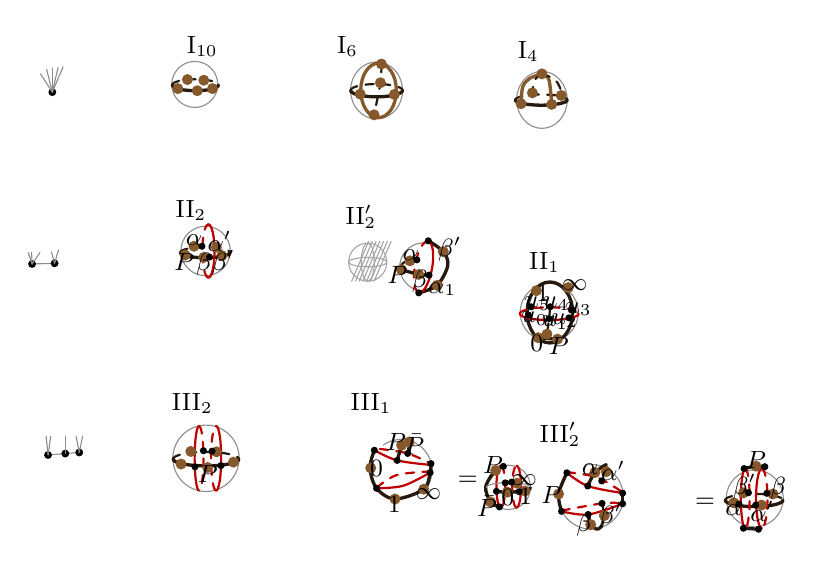
\begin{tikzpicture}[x=1mm,y=-1mm,line cap=round,line join=round,font=\small]
% I_10
\node at (24.13,1.63) {$\mathrm{I}_{10}$};
\draw[pencil] (23.17,6.41) circle[radius=2.92];
\draw[very thick,black!80!brown] plot[smooth, tension=0.55] coordinates {(26.18,6.48) (26.12,6.62) (25.96,6.76) (25.69,6.89) (25.32,7) (24.88,7.09) (24.37,7.15) (23.82,7.19) (23.25,7.21) (22.68,7.19) (22.13,7.15) (21.62,7.09) (21.18,7) (20.81,6.89) (20.54,6.76) (20.38,6.62) (20.32,6.48)};
\draw[thick,dashed,black!80!brown] plot[smooth, tension=0.55] coordinates {(20.32,6.48) (20.38,6.34) (20.54,6.2) (20.81,6.08) (21.18,5.97) (21.62,5.88) (22.13,5.81) (22.68,5.77) (23.25,5.76) (23.82,5.77) (24.37,5.81) (24.88,5.88) (25.32,5.97) (25.69,6.08) (25.96,6.2) (26.12,6.34) (26.18,6.48)};
\fill[Br] (22.24,5.79) circle[radius=0.7];
\fill[Br] (24.32,5.88) circle[radius=0.7];
\fill[Br] (21.02,6.94) circle[radius=0.7];
\fill[Br] (23.49,7.21) circle[radius=0.7];
\fill[Br] (25.42,6.94) circle[radius=0.7];
% I_6
\node at (42.56,1.63) {$\mathrm{I}_{6}$};
\draw[pencil] (46.26,7.17) ellipse[x radius=3.3, y radius=3.62];
\draw[very thick,black!80!brown] plot[smooth, tension=0.55] coordinates {(49.56,7.17) (49.5,7.33) (49.31,7.48) (49,7.62) (48.59,7.74) (48.09,7.85) (47.52,7.92) (46.91,7.97) (46.26,7.98) (45.62,7.97) (45,7.92) (44.43,7.85) (43.93,7.74) (43.52,7.62) (43.22,7.48) (43.03,7.33) (42.96,7.17)};
\draw[thick,dashed,black!80!brown] plot[smooth, tension=0.55] coordinates {(42.96,7.17) (43.03,7.01) (43.22,6.86) (43.52,6.72) (43.93,6.6) (44.43,6.5) (45,6.42) (45.62,6.38) (46.26,6.36) (46.91,6.38) (47.52,6.42) (48.09,6.5) (48.59,6.6) (49,6.72) (49.31,6.86) (49.5,7.01) (49.56,7.17)};
\draw[Br,very thick] (46.51,7.17) ellipse[x radius=2.26, y radius=3.45];
\draw[thick,dashed,black!80!brown] plot[smooth, tension=0.55] coordinates {(46.88,3.82) (46.75,6.2) (45.94,10.27)};
\fill[Br] (46.88,3.82) circle[radius=0.7];
\fill[Br] (46.75,6.2) circle[radius=0.7];
\fill[Br] (44.18,7.64) circle[radius=0.7];
\fill[Br] (48.52,7.68) circle[radius=0.7];
\fill[Br] (45.94,10.27) circle[radius=0.7];
% I_4
\node at (65.52,2.24) {$\mathrm{I}_{4}$};
\draw[pencil] (67.26,8.37) ellipse[x radius=3.21, y radius=3.62];
\draw[very thick,black!80!brown] plot[smooth, tension=0.55] coordinates {(70.48,8.37) (70.41,8.5) (70.23,8.63) (69.92,8.74) (69.51,8.85) (69.01,8.93) (68.44,8.99) (67.82,9.03) (67.18,9.05) (66.54,9.03) (65.92,8.99) (65.35,8.93) (64.85,8.85) (64.44,8.74) (64.13,8.63) (63.94,8.5) (63.88,8.37)};
\draw[thick,dashed,black!80!brown] plot[smooth, tension=0.55] coordinates {(63.88,8.37) (63.94,8.24) (64.13,8.11) (64.44,7.99) (64.85,7.89) (65.35,7.8) (65.92,7.74) (66.54,7.7) (67.18,7.69) (67.82,7.7) (68.44,7.74) (69.01,7.8) (69.51,7.89) (69.92,7.99) (70.23,8.11) (70.41,8.24) (70.48,8.37)};
\draw[Br,very thick] plot[smooth, tension=0.55] coordinates {(64.61,8.86) (64.82,6.73) (65.71,5.64) (67.26,5.07)};
\draw[Br,very thick] plot[smooth, tension=0.55] coordinates {(67.26,5.07) (68.15,5.81) (68.5,8.94)};
\draw[thick,dashed,black!80!brown] plot[smooth, tension=0.55] coordinates {(67.26,5.07) (66.31,5.89) (66.05,7.48)};
\draw[thick,dashed,black!80!brown] plot[smooth, tension=0.55] coordinates {(67.26,5.07) (68.81,5.72) (69.52,6.73) (69.71,7.81)};
\fill[Br] (67.26,5.07) circle[radius=0.7];
\fill[Br] (66.05,7.48) circle[radius=0.7];
\fill[Br] (69.71,7.81) circle[radius=0.7];
\fill[Br] (64.61,8.86) circle[radius=0.7];
\fill[Br] (68.5,8.94) circle[radius=0.7];
% II_2
\node at (22.68,22.38) {$\mathrm{II}_{2}$};
\draw[pencil] (24.54,27.56) circle[radius=3.14];
\draw[very thick,black!80!brown] plot[smooth, tension=0.55] coordinates {(27.63,27.75) (27.57,27.88) (27.39,28.01) (27.1,28.12) (26.71,28.23) (26.23,28.31) (25.69,28.37) (25.1,28.41) (24.49,28.43) (23.87,28.41) (23.29,28.37) (22.74,28.31) (22.27,28.23) (21.87,28.12) (21.58,28.01) (21.41,27.88) (21.35,27.75)};
\draw[thick,dashed,black!80!brown] plot[smooth, tension=0.55] coordinates {(21.35,27.75) (21.41,27.61) (21.58,27.49) (21.87,27.37) (22.27,27.27) (22.74,27.18) (23.29,27.12) (23.87,27.08) (24.49,27.07) (25.1,27.08) (25.69,27.12) (26.23,27.18) (26.71,27.27) (27.1,27.37) (27.39,27.49) (27.57,27.61) (27.63,27.75)};
\draw[Rd,thick] plot[smooth, tension=0.55] coordinates {(24.9,24.18) (25.06,24.25) (25.2,24.44) (25.33,24.75) (25.45,25.17) (25.55,25.68) (25.62,26.27) (25.66,26.9) (25.68,27.56) (25.66,28.22) (25.62,28.86) (25.55,29.44) (25.45,29.95) (25.33,30.37) (25.2,30.69) (25.06,30.88) (24.9,30.94)};
\draw[Rd,thick,dashed] plot[smooth, tension=0.55] coordinates {(24.9,30.94) (24.75,30.88) (24.61,30.69) (24.47,30.37) (24.36,29.95) (24.26,29.44) (24.19,28.86) (24.15,28.22) (24.13,27.56) (24.15,26.9) (24.19,26.27) (24.26,25.68) (24.36,25.17) (24.47,24.75) (24.61,24.44) (24.75,24.25) (24.9,24.18)};
\fill[Br] (23.07,26.96) circle[radius=0.7];
\fill[Br] (25.9,27.07) circle[radius=0.7];
\fill[Br] (21.94,28.08) circle[radius=0.7];
\fill[Br] (24.32,28.37) circle[radius=0.7];
\fill[Br] (26.61,28.15) circle[radius=0.7];
\fill (24.08,26.96) circle[radius=0.45];
\fill (25.05,28.34) circle[radius=0.45];
\node at (23.07,26.18) {$\alpha$};
\node at (26.31,26.35) {$\alpha'$};
\node at (21.85,28.96) {$P$};
\node at (24.35,29.21) {$\beta$};
\node at (26.79,29.04) {$\beta'$};
% struck sphere before II'_2 (hatched over on the page)
\draw[struck] (45.14,28.98) circle[radius=2.42];
\draw[struck] plot[smooth, tension=0.55] coordinates {(47.56,28.98) (47.51,29.1) (47.36,29.21) (47.13,29.32) (46.81,29.41) (46.42,29.48) (45.98,29.53) (45.51,29.56) (45.02,29.57) (44.54,29.55) (44.08,29.51) (43.66,29.45) (43.31,29.36) (43.03,29.26) (42.84,29.15) (42.74,29.04) (42.74,28.92) (42.84,28.8) (43.03,28.69) (43.31,28.59) (43.66,28.51) (44.08,28.44) (44.54,28.4) (45.02,28.38) (45.51,28.39) (45.98,28.42) (46.42,28.47) (46.81,28.54) (47.13,28.64) (47.36,28.74) (47.51,28.86) (47.56,28.98)};
\draw[struck] (45.14,28.98) ellipse[x radius=0.83, y radius=2.42];
\draw[struck] (43.1,31.4) -- (45.24,26.35);
\draw[struck] (43.57,31.4) -- (45.71,26.35);
\draw[struck] (44.05,31.4) -- (46.19,26.35);
\draw[struck] (44.52,31.4) -- (46.67,26.35);
\draw[struck] (45,31.4) -- (47.14,26.35);
\draw[struck] (45.48,31.4) -- (47.62,26.35);
\draw[struck] (45.95,31.4) -- (48.1,26.35);
% II'_2
\node at (44.27,23.23) {$\mathrm{II}'_{2}$};
\draw[pencil] plot[smooth, tension=0.55] coordinates {(52,32.63) (51.39,32.52) (50.83,32.29) (50.32,31.95) (49.89,31.51) (49.55,31) (49.32,30.43) (49.21,29.83) (49.22,29.22) (49.36,28.62) (49.6,28.07) (49.96,27.57) (50.41,27.15) (50.93,26.83) (51.5,26.62) (52.1,26.53) (52.72,26.56) (53.31,26.71)};
\draw[very thick,black!80!brown] plot[smooth, tension=0.55] coordinates {(52.83,26.27) (54.73,27.65) (55.3,29.43) (53.95,31.92) (51.62,32.88)};
\draw[Rd,thick] plot[smooth, tension=0.55] coordinates {(52.8,26.32) (53,26.42) (53.17,26.64) (53.3,26.98) (53.4,27.41) (53.44,27.93) (53.44,28.51) (53.4,29.13) (53.3,29.77) (53.17,30.4) (53,31.01) (52.8,31.55) (52.58,32.02) (52.35,32.4) (52.11,32.67) (51.87,32.82) (51.65,32.84)};
\draw[Rd,thick,dashed] plot[smooth, tension=0.55] coordinates {(51.65,32.84) (51.45,32.74) (51.28,32.52) (51.15,32.19) (51.06,31.75) (51.01,31.23) (51.01,30.65) (51.06,30.03) (51.15,29.39) (51.28,28.76) (51.45,28.16) (51.65,27.61) (51.87,27.14) (52.1,26.77) (52.34,26.5) (52.58,26.35) (52.8,26.32)};
\draw[very thick,black!80!brown] plot[smooth, tension=0.55] coordinates {(49.42,29.94) (51.62,30.54) (52.92,30.63)};
\draw[thick,dashed,black!80!brown] plot[smooth, tension=0.55] coordinates {(49.35,29.46) (49.7,29.04) (50.5,28.81)};
\draw[very thick,black!80!brown] (50.5,28.81) -- (51.38,28.69);
\fill[Br] (50.5,28.81) circle[radius=0.7];
\fill[Br] (54.73,27.65) circle[radius=0.7];
\fill[Br] (49.42,29.94) circle[radius=0.7];
\fill[Br] (51.62,30.54) circle[radius=0.7];
\fill[Br] (53.95,31.92) circle[radius=0.7];
\fill (52.83,26.27) circle[radius=0.45];
\fill (51.62,32.88) circle[radius=0.45];
\fill (52.92,30.63) circle[radius=0.45];
\fill (51.38,28.69) circle[radius=0.45];
\node at (50.6,28.03) {$\alpha$};
\node at (55.54,27.36) {$\beta'$};
\node at (48.93,30.64) {$P$};
\node at (51.73,31.4) {$\beta$};
\node at (54.58,32.41) {$\alpha_1$};
% II_1
\node at (67.58,28.98) {$\mathrm{II}_{1}$};
\draw[pencil] (68.19,35.37) circle[radius=3.69];
\draw[very thick,black!80!brown] (68.27,35.37) ellipse[x radius=2.89, y radius=3.87];
\draw[Rd,thick] plot[smooth, tension=0.55] coordinates {(71.93,35.53) (71.86,35.68) (71.64,35.84) (71.3,35.98) (70.83,36.1) (70.27,36.2) (69.62,36.27) (68.92,36.32) (68.19,36.34) (67.46,36.32) (66.76,36.27) (66.11,36.2) (65.55,36.1) (65.08,35.98) (64.74,35.84) (64.52,35.68) (64.45,35.53)};
\draw[Rd,thick,dashed] plot[smooth, tension=0.55] coordinates {(64.45,35.53) (64.52,35.37) (64.74,35.22) (65.08,35.08) (65.55,34.95) (66.11,34.85) (66.76,34.78) (67.46,34.73) (68.19,34.72) (68.92,34.73) (69.62,34.78) (70.27,34.85) (70.83,34.95) (71.3,35.08) (71.64,35.22) (71.86,35.37) (71.93,35.53)};
\draw[thick,dashed,black!80!brown] plot[smooth, tension=0.55] coordinates {(68.31,34.65) (68.17,36.15) (67.9,38.12)};
\draw[very thick,black!80!brown] (66.77,38.57) -- (69.24,38.76);
\fill[Br] (66.56,32.6) circle[radius=0.7];
\fill[Br] (70.61,32.21) circle[radius=0.7];
\fill[Br] (66.77,38.57) circle[radius=0.7];
\fill[Br] (69.24,38.76) circle[radius=0.7];
\fill[Br] (67.9,38.12) circle[radius=0.7];
\fill (65.9,34.65) circle[radius=0.45];
\fill (68.31,34.65) circle[radius=0.45];
\fill (71.12,35.05) circle[radius=0.45];
\fill (65.54,35.69) circle[radius=0.45];
\fill (68.17,36.15) circle[radius=0.45];
\fill (70.69,36.05) circle[radius=0.45];
\node at (67.38,33) {$1$};
\node at (71.43,31.91) {$\infty$};
\node at (66.67,34.26) {$u_5$};
\node at (69.05,34.26) {$u_4$};
\node at (71.9,34.94) {$u_3$};
\node at (66.31,36.2) {$u_0$};
\node at (68.93,36.62) {$u_1$};
\node at (70.12,36.45) {$u_2$};
\node at (66.61,39.31) {$0$};
\node at (69.4,39.57) {$P$};
% III_2
\node at (22.86,46.97) {$\mathrm{III}_{2}$};
\draw[pencil] (24.6,53.89) circle[radius=4.21];
\draw[very thick,black!80!brown] plot[smooth, tension=0.55] coordinates {(28.77,53.98) (28.69,54.15) (28.46,54.32) (28.07,54.47) (27.55,54.6) (26.92,54.71) (26.19,54.79) (25.41,54.84) (24.6,54.86) (23.78,54.84) (23,54.79) (22.27,54.71) (21.64,54.6) (21.12,54.47) (20.73,54.32) (20.5,54.15) (20.42,53.98)};
\draw[thick,dashed,black!80!brown] plot[smooth, tension=0.55] coordinates {(20.42,53.98) (20.5,53.81) (20.73,53.64) (21.12,53.49) (21.64,53.36) (22.27,53.25) (23,53.16) (23.78,53.11) (24.6,53.1) (25.41,53.11) (26.19,53.16) (26.92,53.25) (27.55,53.36) (28.07,53.49) (28.46,53.64) (28.69,53.81) (28.77,53.98)};
\draw[Rd,thick] plot[smooth, tension=0.55] coordinates {(23.71,57.99) (23.61,57.91) (23.5,57.68) (23.4,57.3) (23.32,56.79) (23.25,56.17) (23.2,55.46) (23.17,54.69) (23.15,53.89) (23.17,53.1) (23.2,52.33) (23.25,51.62) (23.32,51) (23.4,50.49) (23.5,50.11) (23.61,49.88) (23.71,49.8)};
\draw[Rd,thick,dashed] plot[smooth, tension=0.55] coordinates {(23.71,49.8) (23.82,49.88) (23.93,50.11) (24.03,50.49) (24.11,51) (24.18,51.62) (24.23,52.33) (24.26,53.1) (24.27,53.89) (24.26,54.69) (24.23,55.46) (24.18,56.17) (24.11,56.79) (24.03,57.3) (23.93,57.68) (23.82,57.91) (23.71,57.99)};
\draw[Rd,thick] plot[smooth, tension=0.55] coordinates {(25.88,49.8) (26.01,49.88) (26.13,50.11) (26.24,50.49) (26.34,51) (26.42,51.62) (26.47,52.33) (26.51,53.1) (26.52,53.89) (26.51,54.69) (26.47,55.46) (26.42,56.17) (26.34,56.79) (26.24,57.3) (26.13,57.68) (26.01,57.91) (25.88,57.99)};
\draw[Rd,thick,dashed] plot[smooth, tension=0.55] coordinates {(25.88,57.99) (25.76,57.91) (25.63,57.68) (25.52,57.3) (25.43,56.79) (25.35,56.17) (25.29,55.46) (25.25,54.69) (25.24,53.89) (25.25,53.1) (25.29,52.33) (25.35,51.62) (25.43,51) (25.52,50.49) (25.63,50.11) (25.76,49.88) (25.88,49.8)};
\fill[Br] (22.67,53.02) circle[radius=0.7];
\fill[Br] (25.93,53.07) circle[radius=0.7];
\fill[Br] (21.43,54.62) circle[radius=0.7];
\fill[Br] (24.79,55.06) circle[radius=0.7];
\fill[Br] (28.08,54.38) circle[radius=0.7];
\fill (24.27,52.93) circle[radius=0.45];
\fill (25.36,52.99) circle[radius=0.45];
\fill (23.2,54.97) circle[radius=0.45];
\fill (26.5,54.82) circle[radius=0.45];
\node at (24.82,55.9) {$P$};
% III_1 and its twin
\node at (45.56,46.97) {$\mathrm{III}_{1}$};
\draw[pencil] plot[smooth, tension=0.55] coordinates {(47.1,52.22) (47.78,51.83) (48.52,51.59) (49.29,51.5) (50.06,51.57) (50.81,51.78) (51.5,52.14) (52.11,52.62) (52.61,53.22) (52.98,53.9) (53.22,54.65) (53.3,55.42) (53.23,56.2) (53,56.94) (52.64,57.63) (52.14,58.23)};
\draw[very thick,black!80!brown] plot[smooth, tension=0.55] coordinates {(45.98,52.87) (45.42,55.12) (46.26,57.7) (48.6,59.06) (52.25,57.82) (53.06,55.71) (53.17,54.57)};
\draw[Rd,thick] plot[smooth, tension=0.55] coordinates {(45.98,52.87) (48.87,54.16) (53.17,54.74)};
\draw[Rd,thick,dashed] plot[smooth, tension=0.55] coordinates {(46.67,52.7) (50.21,53.27) (53.17,54.57)};
\draw[Rd,thick] plot[smooth, tension=0.55] coordinates {(46.26,57.7) (49.64,57.38) (53.06,55.71)};
\draw[Rd,thick,dashed] plot[smooth, tension=0.55] coordinates {(46.26,57.62) (48.81,56.02) (53.06,55.56)};
\draw[very thick,black!80!brown] (49.44,52.23) -- (48.87,54.16);
\draw[thick,dashed,black!80!brown] (50.4,51.82) -- (50.21,53.27);
\fill[Br] (49.44,52.23) circle[radius=0.7];
\fill[Br] (50.4,51.82) circle[radius=0.7];
\fill[Br] (45.52,55.12) circle[radius=0.7];
\fill[Br] (52.25,57.82) circle[radius=0.7];
\fill[Br] (48.6,59.06) circle[radius=0.7];
\fill (45.98,52.87) circle[radius=0.45];
\fill (48.87,54.16) circle[radius=0.45];
\fill (50.21,53.27) circle[radius=0.45];
\fill (53.17,54.57) circle[radius=0.45];
\fill (53.06,55.71) circle[radius=0.45];
\fill (46.26,57.7) circle[radius=0.45];
\node at (48.75,51.86) {$P$};
\node at (51.07,52.11) {$\bar P$};
\node at (46.25,55.14) {$0$};
\node at (52.86,58.42) {$\infty$};
\node at (48.51,59.77) {$1$};
\node at (57.85,56.77) {$=$};
\draw[pencil] (63,57.58) circle[radius=2.81];
\draw[very thick,black!80!brown] plot[smooth, tension=0.55] coordinates {(62.36,54.92) (61.39,55.43) (60.12,57.5) (60.75,59.45) (61.87,60.07)};
\draw[Rd,thick] plot[smooth, tension=0.55] coordinates {(62.04,60.15) (61.93,60.1) (61.82,59.95) (61.72,59.7) (61.64,59.37) (61.57,58.97) (61.52,58.51) (61.49,58.02) (61.48,57.5) (61.49,56.98) (61.52,56.48) (61.57,56.02) (61.64,55.62) (61.72,55.29) (61.82,55.04) (61.93,54.89) (62.04,54.84)};
\draw[Rd,thick,dashed] plot[smooth, tension=0.55] coordinates {(62.04,54.84) (62.14,54.89) (62.25,55.04) (62.35,55.29) (62.43,55.62) (62.5,56.02) (62.55,56.48) (62.58,56.98) (62.6,57.5) (62.58,58.02) (62.55,58.51) (62.5,58.97) (62.43,59.37) (62.35,59.7) (62.25,59.95) (62.14,60.1) (62.04,60.15)};
\draw[Rd,thick] plot[smooth, tension=0.55] coordinates {(64.05,54.84) (64.16,54.89) (64.26,55.04) (64.36,55.29) (64.44,55.62) (64.51,56.02) (64.56,56.48) (64.6,56.98) (64.61,57.5) (64.6,58.02) (64.56,58.51) (64.51,58.97) (64.44,59.37) (64.36,59.7) (64.26,59.95) (64.16,60.1) (64.05,60.15)};
\draw[Rd,thick,dashed] plot[smooth, tension=0.55] coordinates {(64.05,60.15) (63.94,60.1) (63.83,59.95) (63.74,59.7) (63.65,59.37) (63.58,58.97) (63.53,58.51) (63.5,58.02) (63.49,57.5) (63.5,56.98) (63.53,56.48) (63.58,56.02) (63.65,55.62) (63.74,55.29) (63.83,55.04) (63.94,54.89) (64.05,54.84)};
\draw[pencil] plot[smooth, tension=0.55] coordinates {(60.19,57.58) (60.24,57.47) (60.4,57.35) (60.66,57.25) (61.01,57.16) (61.44,57.09) (61.92,57.03) (62.45,57) (63,56.99) (63.55,57) (64.08,57.03) (64.56,57.09) (64.99,57.16) (65.34,57.25) (65.6,57.35) (65.76,57.47) (65.81,57.58)};
\draw[very thick,black!80!brown] plot[smooth, tension=0.55] coordinates {(61.48,58.09) (62.87,58.19) (65.1,58.05) (65.81,57.67)};
\draw[very thick,black!80!brown] (62.6,57.01) -- (63.4,56.92);
\draw[thick,dashed,black!80!brown] (63.4,56.92) -- (64.64,57.03);
\fill[Br] (61.39,55.43) circle[radius=0.7];
\fill[Br] (60.75,59.45) circle[radius=0.7];
\fill[Br] (62.87,58.19) circle[radius=0.7];
\fill[Br] (65.1,58.05) circle[radius=0.7];
\fill[Br] (64.1,57.06) circle[radius=0.7];
\fill (62.36,54.92) circle[radius=0.45];
\fill (61.87,60.07) circle[radius=0.45];
\fill (61.48,58.09) circle[radius=0.45];
\fill (64.37,58.14) circle[radius=0.45];
\fill (62.6,57.01) circle[radius=0.45];
\fill (63.4,56.92) circle[radius=0.45];
\node at (61.07,54.8) {$P$};
\node at (60.3,60.02) {$\bar P$};
\node at (62.92,58.84) {$0$};
\node at (65.18,58.68) {$1$};
\node at (65,56.66) {$\infty$};
% III'_2 and its twin
\node at (69.56,50.85) {$\mathrm{III}'_{2}$};
\draw[pencil] plot[smooth, tension=0.55] coordinates {(72.77,54.73) (73.62,54.67) (74.47,54.79) (75.27,55.08) (76,55.52) (76.61,56.11) (77.1,56.81) (77.42,57.6) (77.58,58.44) (77.56,59.29) (77.37,60.12) (77.01,60.89) (76.5,61.57) (75.86,62.13) (75.11,62.55) (74.3,62.8) (73.45,62.88) (72.61,62.79) (71.8,62.52) (71.06,62.09) (70.43,61.52) (69.93,60.83)};
\draw[very thick,black!80!brown] plot[smooth, tension=0.55] coordinates {(70.43,55.73) (69.38,58.42) (69.75,60.63)};
\draw[Rd,thick] plot[smooth, tension=0.55] coordinates {(70.43,55.73) (73.08,57.41) (77.51,58.31)};
\draw[Rd,thick,dashed] plot[smooth, tension=0.55] coordinates {(70.43,55.65) (74.29,56.32) (77.51,58.22)};
\draw[Rd,thick] plot[smooth, tension=0.55] coordinates {(69.75,60.63) (73.13,61.03) (77.51,59.67)};
\draw[Rd,thick,dashed] plot[smooth, tension=0.55] coordinates {(69.75,60.54) (74.89,59.62) (77.51,59.59)};
\draw[very thick,black!80!brown] (77.51,58.31) -- (77.51,59.67);
\draw[very thick,black!80!brown] plot[smooth, tension=0.55] coordinates {(73.08,57.41) (73.98,55.7) (75.42,54.69)};
\draw[thick,dashed,black!80!brown] plot[smooth, tension=0.55] coordinates {(75.42,54.69) (75.42,55.59) (74.86,56.77)};
\draw[very thick,black!80!brown] plot[smooth, tension=0.55] coordinates {(73.13,61.03) (73.45,62.31) (74.29,62.89) (74.88,62.46)};
\draw[thick,dashed,black!80!brown] plot[smooth, tension=0.55] coordinates {(74.88,62.46) (75.18,61.17) (74.89,59.62)};
\fill[Br] (69.38,58.42) circle[radius=0.7];
\fill[Br] (73.98,55.7) circle[radius=0.7];
\fill[Br] (75.42,55.59) circle[radius=0.7];
\fill[Br] (73.45,62.31) circle[radius=0.7];
\fill[Br] (75.18,61.17) circle[radius=0.7];
\fill (70.43,55.73) circle[radius=0.45];
\fill (73.08,57.41) circle[radius=0.45];
\fill (74.86,56.77) circle[radius=0.45];
\fill (77.51,58.31) circle[radius=0.45];
\fill (77.51,59.67) circle[radius=0.45];
\fill (69.75,60.63) circle[radius=0.45];
\fill (73.13,61.03) circle[radius=0.45];
\fill (74.89,59.62) circle[radius=0.45];
\node at (68.45,58.59) {$P$};
\node at (73.39,55.31) {$\alpha$};
\node at (76.31,55.48) {$\alpha'$};
\node at (72.62,62.38) {$\beta$};
\node at (76.01,61.2) {$\beta'$};
\node at (87.98,59.6) {$=$};
\draw[pencil] (94.29,58.98) circle[radius=3.62];
\draw[very thick,black!80!brown] plot[smooth, tension=0.55] coordinates {(92.93,55.19) (94.45,54.89) (95.57,54.96)};
\draw[very thick,black!80!brown] (92.85,62.77) -- (94.77,62.9);
\draw[very thick,black!80!brown] plot[smooth, tension=0.55] coordinates {(97.87,59.21) (97.8,59.37) (97.59,59.52) (97.25,59.66) (96.8,59.79) (96.24,59.89) (95.61,59.96) (94.92,60.01) (94.2,60.02) (93.49,60.01) (92.8,59.96) (92.17,59.89) (91.61,59.79) (91.15,59.66) (90.81,59.52) (90.61,59.37) (90.54,59.21)};
\draw[thick,dashed,black!80!brown] plot[smooth, tension=0.55] coordinates {(90.54,59.21) (90.61,59.06) (90.81,58.9) (91.15,58.77) (91.61,58.64) (92.17,58.54) (92.8,58.47) (93.49,58.42) (94.2,58.41) (94.92,58.42) (95.61,58.47) (96.24,58.54) (96.8,58.64) (97.25,58.77) (97.59,58.9) (97.8,59.06) (97.87,59.21)};
\draw[Rd,thick] plot[smooth, tension=0.55] coordinates {(93.08,62.75) (92.97,62.68) (92.87,62.47) (92.77,62.12) (92.69,61.65) (92.62,61.08) (92.57,60.42) (92.53,59.72) (92.52,58.98) (92.53,58.24) (92.57,57.53) (92.62,56.88) (92.69,56.31) (92.77,55.84) (92.87,55.49) (92.97,55.28) (93.08,55.21)};
\draw[Rd,thick,dashed] plot[smooth, tension=0.55] coordinates {(93.08,55.21) (93.19,55.28) (93.3,55.49) (93.39,55.84) (93.48,56.31) (93.55,56.88) (93.6,57.53) (93.63,58.24) (93.64,58.98) (93.63,59.72) (93.6,60.42) (93.55,61.08) (93.48,61.65) (93.39,62.12) (93.3,62.47) (93.19,62.68) (93.08,62.75)};
\draw[Rd,thick] plot[smooth, tension=0.55] coordinates {(95.18,62.75) (95.04,62.68) (94.9,62.47) (94.78,62.12) (94.67,61.65) (94.57,61.08) (94.51,60.42) (94.47,59.72) (94.45,58.98) (94.47,58.24) (94.51,57.53) (94.57,56.88) (94.67,56.31) (94.78,55.84) (94.9,55.49) (95.04,55.28) (95.18,55.21)};
\draw[Rd,thick,dashed] plot[smooth, tension=0.55] coordinates {(95.18,55.21) (95.32,55.28) (95.46,55.49) (95.58,55.84) (95.69,56.31) (95.78,56.88) (95.85,57.53) (95.89,58.24) (95.9,58.98) (95.89,59.72) (95.85,60.42) (95.78,61.08) (95.69,61.65) (95.58,62.12) (95.46,62.47) (95.32,62.68) (95.18,62.75)};
\fill[Br] (94.45,54.89) circle[radius=0.7];
\fill[Br] (92.85,58.29) circle[radius=0.7];
\fill[Br] (96.6,58.42) circle[radius=0.7];
\fill[Br] (91.63,59.55) circle[radius=0.7];
\fill[Br] (95.14,59.84) circle[radius=0.7];
\fill (92.93,55.19) circle[radius=0.45];
\fill (95.57,54.96) circle[radius=0.45];
\fill (93.49,58.26) circle[radius=0.45];
\fill (95.82,58.34) circle[radius=0.45];
\fill (92.27,59.7) circle[radius=0.45];
\fill (94.4,59.84) circle[radius=0.45];
\fill (92.85,62.77) circle[radius=0.45];
\fill (94.77,62.9) circle[radius=0.45];
\node at (94.45,54.05) {$P$};
\node at (92.98,57.5) {$\beta'$};
\node at (97.26,57.75) {$\beta$};
\node at (91.61,60.44) {$\alpha$};
\node at (95.24,60.61) {$\alpha'$};
% three marginal graphs
\fill (5.08,7.39) circle[radius=0.5];
\draw[pencil] (5.08,7.39) -- (3.56,5.05);
\draw[pencil] (5.08,7.39) -- (4.36,4.5);
\draw[pencil] (5.08,7.39) -- (5.08,4.31);
\draw[pencil] (5.08,7.39) -- (5.81,4.26);
\draw[pencil] (5.08,7.39) -- (6.45,4.18);
\draw[pencil] (2.51,29.21) -- (5.37,29.13);
\fill (2.51,29.21) circle[radius=0.5];
\fill (5.37,29.13) circle[radius=0.5];
\draw[pencil] (2.51,29.21) -- (2.02,27.78);
\draw[pencil] (2.51,29.21) -- (2.44,27.73);
\draw[pencil] (2.51,29.21) -- (3.52,27.76);
\draw[pencil] (5.37,29.13) -- (4.98,27.68);
\draw[pencil] (5.37,29.13) -- (5.86,27.44);
\draw[pencil] (4.54,53.47) -- (6.73,53.29);
\draw[pencil] (6.73,53.29) -- (8.5,53.15);
\fill (4.54,53.47) circle[radius=0.5];
\fill (6.73,53.29) circle[radius=0.5];
\fill (8.5,53.15) circle[radius=0.5];
\draw[pencil] (4.54,53.47) -- (4.29,51.1);
\draw[pencil] (4.54,53.47) -- (4.88,51.1);
\draw[pencil] (6.73,53.29) -- (6.73,51.1);
\draw[pencil] (8.5,53.15) -- (8.1,51.1);
\draw[pencil] (8.5,53.15) -- (8.93,51.1);
\end{tikzpicture}
\end{document}
